\documentclass[11pt]{article}
\usepackage[utf8]{inputenc}
\usepackage{url}
\usepackage{color,hyperref}
\usepackage{listings}
\usepackage{subcaption}
\usepackage{graphicx}
\usepackage{seqsplit}

\title{cNMA Usage Documentation}

\begin{document}
\author{Tomasz Oliwa, Haoran Chen\\
		\href{mailto:cnma.shenlab@gmail.com}{cnma.shenlab@gmail.com}}

   \lstset{language=bash,
		   basicstyle=\ttfamily\scriptsize,
		   breaklines=true
		  }
\maketitle




\begin{abstract}
This is the work in progress documentation for the cNMA set of scripts. It containts usage hints for a user points of view.
\end{abstract}

\begin{figure}[h]
\centering
{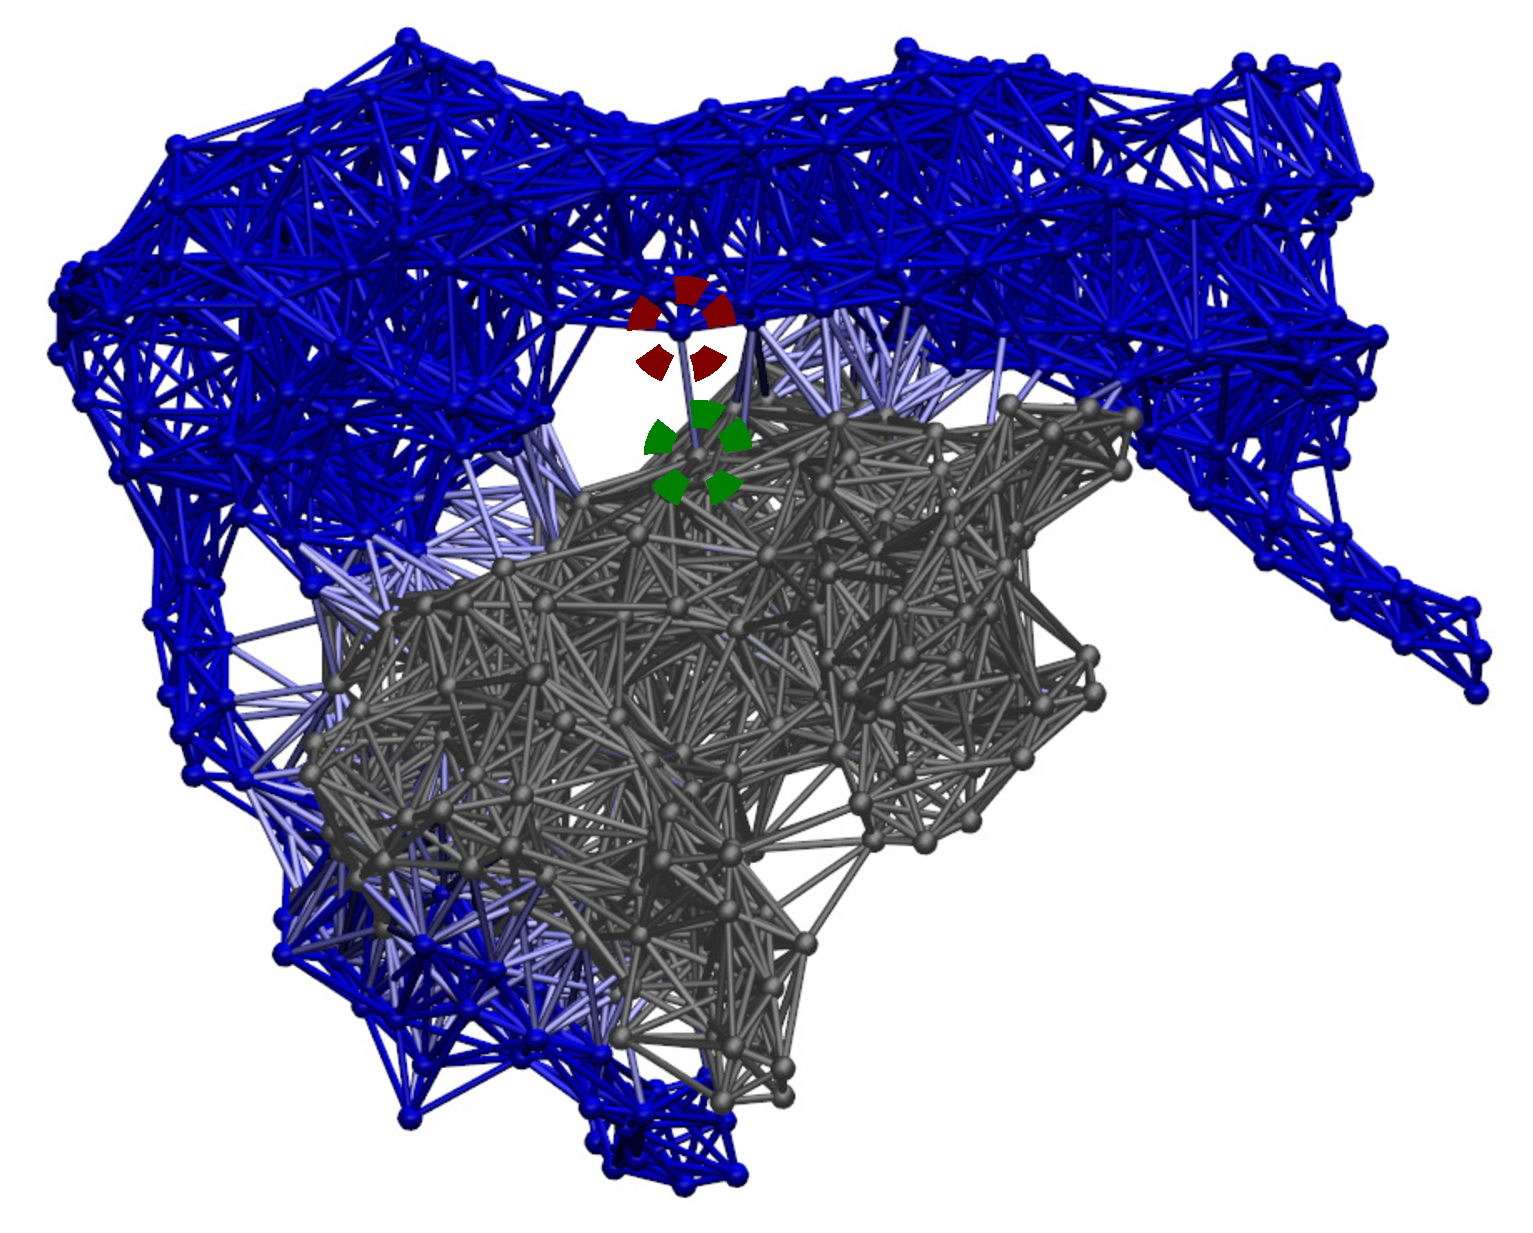
\includegraphics[width=10cm]{pics/cnma.eps}}
\end{figure}
\newpage
\tableofcontents

\clearpage

% \section{How to update the manual}
% The manual is written as a *.tex file and can be compiled with ``pdflatex'' to generate a ``*.pdf'' file as follows:

% \begin{lstlisting}
% $ pdflatex nmamanual1.tex
% \end{lstlisting}

% With the program ``hevea'', a HTML version of the manual including all pictures and illustrations is possible as follows:

% \begin{lstlisting}
% $ hevea nmamanual1.tex
% $ imagen nmamanual1
% $ hevea nmamanual1.tex
% \end{lstlisting}

% The command above will generate a ``*.html'' file. The ``hevea'' command might complain that the ``seqsplit'' command has not been found as: ``Command not found: \\seqsplit''. This is normal, the ``seqsplit'' command is used for the PDF version of this manual. It forces an automatic line break of long names that would otherwise go beyond the margin of a PDF page. With hevea, a HTML version is generated which is not bound by horizontal page margins, and ``seqsplit'' is not necessary.

\section{cNMA Prerequisites}
The prerequisites for cNMA are:

\begin{itemize}
 \item Python $>=$ 2.7
 \item ProDy $>=$ 1.5.1 \url{http://prody.csb.pitt.edu/}
 \item NumPy (tested on 1.8.0), SciPy (tested on 0.12.1 and 0.13.3)
 \item Matplotlib
\end{itemize}

\subsection{Anaconda - A collection of prerequisites}

The aforementioned  (except ProDy) were installed on the cluster in userspace through the Anaconda Python package \url{http://continuum.io/downloads}. At the time of writing, the Anaconda package for 64 Bit machines with Python 2.7 version is \seqsplit{``Anaconda2-4.1.1-Linux-x86\_64.sh''} and can be installed through the following commands:

\begin{lstlisting}
$ chmod +x Anaconda2-4.1.1-Linux-x86_64.sh
$ ./Anaconda2-4.1.1-Linux-x86_64.sh
\end{lstlisting}

The will create a about 1.1 GB large directory ``anaconda2'' in the home directory ``~/'', containing the binaries, packages and environments of Python and the libaries. To then run a Python program with the Python interpreter from Anaconda, the path to it should be given in the commandline, such as:

\begin{lstlisting}
$ ~/anaconda2/bin/python x.py
\end{lstlisting}

In this manual, it is assumed that the cNMA and other Python programs are run with the prerequisites installed, and a Python 2.7 interpreter is called either through the Anaconda path or by having it installed otherwise.

Anaconda is fairly large and installs numerous packages. To reduce the needed installation space, the package ``Miniconda'' can be used instead. It is available from \url{http://conda.pydata.org/miniconda.html#miniconda}. Miniconda contains a version of Python and the conda installer, through which specific pre-requisites (such as NumPy) can be obtained. 
Commandline examples to do so can be found on the Miniconda website. 

ProDy itself can be also installed once Anaconda has finished the installation process. Anaconda provides ``pip'', a package manager for Python to do so as follows:

\begin{lstlisting}
$ ~/anaconda2/bin/pip install ProDy
\end{lstlisting}

The pip installation of ProDy will be placed inside the anaconda2 directory.

For Python 3.5 users, the only difference step for the procedure above is that the Anaconda version should be \seqsplit{``Anaconda3-4.1.1-MacOSX-x86\_64.sh''}.

\subsection{Download of cNMA}
cNMA is available on Github at: \url{https://github.tamu.edu/shen-group/cNMA} 

This git repository is (at the time of writing) a private repository. As a member of cNMA, it is possible to give other users access to it through the link ``Invite users to this repo Send invitation'' on aforementioned URL on the top right-hand site.

cNMA can be downloaded through a web browser by clicking ``Download ZIP'' at: \url{https://github.tamu.edu/shen-group/cNMA}

cNMA can be also obtained by using ``Git'' through:

\begin{lstlisting}
$ git clone https://github.tamu.edu/shen-group/cNMA.git
\end{lstlisting}

where ``USER'' should be replaced by the bitbucket username that has access to cNMA. The commandline will promt for the users bitbucket password.

\subsection{Modification to Prerequisites}
Modifications to the ProDy prerequisite have been made and can be found in the folder ``cNMA/Manual/Documentation/modified/''. The modifications are:

\begin{itemize}
 \item ProDy:
   \begin{enumerate}
	\item Add method matchTNMAChains in prody.proteins.compare\\This method defines chain matching based on Bio.pairwise2 from Biopython and forces it. 
	The chain matching method was too deeply rooted in ProDy to create a new one in the NMAUnified programs, hence a method ``matchTNMAChains'' was created based on 
	the ProDy method ``matchChains'' and put into prody.proteins.compare (in the file compare.py)
	\item Bugfix to pass the argument zeros in the method calcANM in prody.dynamics.anm, to calculate trivial normal modes (in the file anm.py)
	\item Addon with the zeros parameter to write trivial normal modes directly with the writeNMD method in prody.dynamics.nmdfile. This addon is not necessary to run the cNMA data collection, as these perform the writing of trivial normal modes into the NMD files via shell scripting and temp files. However, this addon is useful for direct experimentation with ProDy and normal modes (in the file nmdfile.py) to be able to visualize modes directly after calculating them.
   \end{enumerate}
\end{itemize}
\noindent
The files are located in the \path{cNMA/Manual/Documentation/modified/} subfolder of this manual and should be copied over the original ProDy files with the same name.

A script called ``replacePrerequisites.sh'' is provided along with the modified files, which will place them in their right position. To run it, the current work directory should be changed into its folder, the script made executable and then finally run, this is done by the following three commands:

\begin{lstlisting}
$ cd cNMA/Manual/Documentation/modified/
$ chmod +x replacePrerequisites.sh
$ ./replacePrerequisites.sh
\end{lstlisting}

The contents of ``replacePrerequisites.sh'' itself is:
\begin{lstlisting}
#!/bin/bash
cp compare.py ~/anaconda2/lib/python2.7/site-packages/prody/proteins/
cp anm.py ~/anaconda2/lib/python2.7/site-packages/prody/dynamics/
cp nmdfile.py ~/anaconda2/lib/python2.7/site-packages/prody/dynamics/

rm -f ~/anaconda2/lib/python2.7/site-packages/prody/proteins/compare.pyc
rm -f ~/anaconda2/lib/python2.7/site-packages/prody/dynamics/anm.pyc
rm -f ~/anaconda2/lib/python2.7/site-packages/prody/dynamics/nmdfile.pyc
\end{lstlisting}

If Anaconda is installed in a different path then specified by the script above, this path needs to be located to replace the modified .py files.

For instance, on dao the userspace path is \path{~/anaconda2/lib/python2.7/site-packages/prody/} and on the local Fedora machine it is \path{/usr/lib64/python2.7/site-packages/prody/}.

The corresponding *.pyc also need to be deleted so that Python will guarantee to compile the .py file anew. A .pyc file is usually made when the Python .py file is imported by some other script and contains the compiled byte-code of the source file.



\section{Data collection}
\label{sec:data_collection}
Usage overview over how to generate the cNMA results.

\subsection{NMAUnified}
The main program for the cNMA is calculation is ``NMAUnified.py''. Its input are a configuration class describing the experiment and two proteins in PDB format. Its output is written in a folder and contains the experimental results such as RMSD reduction and NMD files. 

\subsubsection{Input}
Running it without arguments prints a help text with usage and argument descriptors:

\begin{lstlisting}
$ python NMAUnified.py
\end{lstlisting}

Ultimatively, NMAUnified expects two arguments in the following order:
\begin{enumerate}
 \item config, the Configurations class
 \item protein1\_A, the Protein 1 in first conformational state
 \item protein2\_A, the Protein 2 in first conformational state
 % \item protein1\_B, the Protein 1 in second conformational state
 % \item protein2\_B, the Protein 2 in second conformational state
\end{enumerate}

In config, the parameters of the experiments are set, each parameter is documented via a comment. Examples of parameters are the output paths, 
the kind of NMA performed or the RMSD fitting precision.

An example of how to run the program with a profiler attached to it is:

\begin{lstlisting}
$ python NMAUnified.py --profile cNMA/Manual/Example/Example1/Input/Configuration.py Manual/Example/Example1/Input/1A2K_r_u.pdb Manual/Example/Example1/Input/1A2K_l_u.pdb
\end{lstlisting}

The optional parameters, such as ``--profile'' for NMAUnified are:

\begin{itemize}
 \item -h, --help            show this help message and exit
 \item --profiler            Run the program with a profiler attached to it, that
						writes runtime information after a successful run.
 \item --outputPath OUTPUTPATH
						Directly specify the output path of the program,
						ignoring the output path in the Configuration
 \item --affirmProteinNames AFFIRMPROTEINNAMES
						If the arguments for protein1\_A, protein2\_A,
						do not follow the xxxx\_r/l\_l/b.pdb naming scheme of
						the Protein-Protein Docking Benchmark 4.0, provide 
						``receptor'' to tell the program that protein1 is a 
						receptor (and protein2 therefore a ligand), or provide
						``ligand'' to state the opposite. The titles of the proteins 
						will be adjusted accordingly.
\end{itemize}

\subsubsection{Output}
The output will be written \seqsplit{outputPath+experimentName}. \\
The variables outputPath and experimentNamePrefix are set in the Configuration file, the experimentName is determined by the filename of the protein inputs. An example from a Configuration.py file can looks as follows:

\begin{verbatim}
# Path to the output
self.outputPath = "/home/usersname/Documents/cNMAoutput/"

# Experiment name prefix to be used to create the results output folder
self.experimentNamePrefix = "results"
		
\end{verbatim}

\subsection{Examples}
\subsubsection{Example 1}

Two pdb files for cNMA can be found in \path{cNMA/Manual/Example/Example1/Input/}. One is 1A2K\_r\_u.pdb as unbound receptor, another is 1A2K\_l\_u.pdb as unbound ligand. After running the command above, the expected output is in the folder \path{cNMA/Manual/Example/Example1/Ouput/}

\subsubsection{Example 2}

One pdb file 1A2K\_r\_u.pdb for canonical NMA can be found in \path{cNMA/Manual/Example/Example2/Input/}. After running the command above, the expected output is in the folder \path{cNMA/Manual/Example/Example2/Ouput/}

\subsubsection{Example 3}

Four pdb files for cNMA with posterior analysis can be found in \path{cNMA/Manual/Example/Example3/Input/}. They are 1A2K\_r\_u.pdb for unbound receptor, 1A2K\_l\_u.pdb for unbound ligand, 1A2K\_r\_b.pdb for bound receptor, and 1A2K\_l\_b.pdb for bound ligand. After running the command above, the expected output is in the folder \path{cNMA/Manual/Example/Example3/Ouput/}

\subsubsection{Configuration}
The Configurations file given to NMAUnified determines the experiment setup. In the following, at first a parameter dictionary for the configuration file is given, followed by a listing of example configuration files accompaning data gathering files.

\subsubsection{Configuration Dictionary}
The parameters (here in \textbf{boldface}) are present in a configuration file. After each parameter, an explanation of it is given here, followed by an example of a set parameter. Parameters with star are for posterior analysis in Example 3.

\begin{itemize}
\item \textbf{self.outputPath}: The path to the output. \\ 
Example: \seqsplit{self.outputPath = ``/home/usersname/Documents/cNMAoutput/''}

\item \textbf{self.experimentNamePrefix}: Experiment name prefix to be used to create the results output folder. \\
% Example: \seqsplit{self.experimentNamePrefix = ``2b\_individual\_2k\_whole\_bb\_HC\_U1\_modelsubmatrix\_d8.0\_gamma0.25\_projectionTrue\_projectionStylefull\_align2bindividual''}
Example: self.experimentNamePrefix = ``result''

\item \textbf{self.investigationsOn}: Data collection on individual proteins or for a complex. Possible values: ``Individual'', ``Complex''. \\
Example: \seqsplit{self.investigationsOn = ``Individual''}

\item \textbf{self.measuresOnWhole}: Data collection on the whole protein/complex if true, else on the interface. Possible values: ``True'', ``False''. \\
Example: \seqsplit{self.measuresOnWhole = True}

\item \textbf{self.calculateZeroEigvalModes}: Calculate zero eigenvalue modes. \\
Example: \seqsplit{self.calculateZeroEigvalModes = True}

\item \textbf{self.align*}: Align styles of unbound to bound. The setting of the aforementioned \textbf{measuresOnWhole} will furthermore determine if the alignment basis is the whole or the interface. Possible values: ``alpha'': align protein1 and protein2 independently, ``beta'' : align protein 1 and rigid bodily ``drag'' protein 2 along, ``complexOnComplex'': align complex on complex, ``2bcomplex'': first align alpha whole to create the complex, then align the complex again based on complexOnComplex, ``2bindividual'': first align alpha whole to create the complex, then align the complex again based on beta of the reference segment for whole or interface \\
Example: \seqsplit{self.align = ``2bindividual''}

\item \textbf{self.complexRMSDreduction*}: The setup of the normal mode array for data gathering, for \textbf{\seqsplit{self.investigationsOn}} set to ``Individual'', choose ``2k'', for investigations on ``Complex'', choose ``2k'' for a cNMA setup to be further specified in the parameter \textbf{\seqsplit{self.whichCustomHC}}, or choose ``1k1k'' or ``1k1k6'' for a conventional NMA setup, the latter enabling six rigid body modes for data gathering RMSD reduction purposes. \\
Example: \seqsplit{self.complexRMSDreduction = ``1k1k6''}

\item \textbf{self.whichCustomHC}: HC setup, for \textbf{\seqsplit{self.investigationsOn}} set to ``Individual'', choose ``HC\_U1''. For \textbf{\seqsplit{self.investigationsOn}} set to ``Complex'', choose ``HC\_U1'' for allowing intermolecular interactions, ``HC\_0'' for not allowing intermolecular interactions, ``HC\_06'' for ``HC\_0'' and 6 trival modes of the ligand as first modes to be used for RMSD reduction calculations, ``HC\_U1\_1k1k'' to calculate modes from ``HC\_U1'', then split them into 1k1k component vectors. \\ 
Example: \seqsplit{self.whichCustomHC = ``HC\_U1''}

\item \textbf{self.filterPDB}: When parsing PDB files, filter by ProDys ``protein'' selection? Without this filtering (set as ``None''), mismatches have occurred. \\
Example: \seqsplit{self.filterPDB = ``protein''}

\item \textbf{self.whatAtomsToMatch*}: What atoms are subject to the matching of chains, Possible values: ``calpha'', ``bb'' or ``all''. \\
Example \seqsplit{self.whatAtomsToMatch = ``bb''}

\item \textbf{self.customH}: Create the modified Hessians or keep conventional/canonical Hessians. If set to ``False'', only canonical NMA will be performed, if set to ``True'', the potential U1 will be used to involve intermolecular interactions. \\
Example: \seqsplit{self.customH = True}

\item \textbf{self.customHRdistance}: Cut-off distance D for intermolecular springs. \\
Example: \seqsplit{self.customHRdistance = 8.0}

\item \textbf{self.customForceConstant} Force constant gamma for intermolecular springs. \\
Example: \seqsplit{self.customForceConstant = 0.25}

\item \textbf{self.whichCustomHIndividual}: Method to obtain the normal modes for the RMSD reduction on \textbf{self.investigationsOn} set to ``Individual'', the valid settings are: ``HC\_subvector'': subvector method, ``submatrix'' : submatrix method, ``canonical'': use normal modes from the canonical individual protein. \\
Example: \seqsplit{self.whichCustomHIndividual = ``submatrix''}

\item \textbf{self.projectHessian}: Use a transformation/projection technique on the Hessian (projection matrix treadment 8.27 NMA book or Non-Eckart body Frame Fuchigami U matrix) is ``True'', else do not use such a technique. \\ 
Example: \seqsplit{self.projectHessian = True}

\item \textbf{self.projectionStyle}: If \textbf{self.projectHessian} is ``True'', define the style of the transformation/projection. Valid settings are ``full'': project away from protein1 part, ``fullComplex'': project away from the whole complex, ``fixedDomainFrame'': use the U transformation matrix to setup the receptor as fixed domain. \\
Example: \seqsplit{self.projectionStyle = ``full''}

\item \textbf{self.rescaleEigenvalues}: Use a re-ranking of eigenvalues, known as the $lambda^{R}$ approach. 
If set to ``True'', eigenvalues are re-ranked via $lambda^{R}$, if set to ``False'', no re-ranking takes place.  \\ 
Example: \seqsplit{self.rescaleEigenvalues = False}

\item \textbf{self.floatingPointThreshold}: Small value to consider skipping the protein investigation if the initial RMSD is not bigger than it. \\
Example: \seqsplit{self.floatingPointThreshold = 0.000000000001}

\item \textbf{self.stopRMSDReductionAt*}: Set the number of maximal normal modes, at which the RMSD reduction based on the Swarmdock betas approach is stopped. To not have any limit/stop, set this to a high value. \\
Example: \seqsplit{self.stopRMSDReductionAt = 400}

\item \textbf{self.maxModesToCalculate}: Upper limit for mode calculation, set to very high number (1000000) to calculate 3n-6 modes. For \textbf{\seqsplit{self.investigationsOn}} set to ``Individual'', this is the number of modes (excluding trivial modes) to be calculated. For \textbf{\seqsplit{self.investigationsOn}} set to ``Complex'', this is the value k, meaning that 2k modes (excluding trivial modes) will be obtained for the complex. \\        
Example: \seqsplit{self.maxModesToCalculate = 400}

\item \textbf{self.precisionBetaFitting*}: Precision for RMSD beta fitting. \\
Example: \seqsplit{self.precisionBetaFitting = 1e-6}

\item \textbf{self.maxIterBetas*}: How many iterations are to be allowed for the betas fitter (Swarmdock approach). \\
Example: \seqsplit{self.maxIterBetas = 60000}
\end{itemize}

% \subsubsection{Configuration Files}
% Inside the ``configuration/'' folder are the following files:

% \begin{itemize}
%  \item Configurations\_NMAUnifiedIndividualTemplate.py: A configuration template with comments on every setting is given in.
%  \item \seqsplit{2b\_individual\_2k\_whole\_bb\_HC\_U1\_modelsubmatrix\_d8.0\_gamma0.25\_projectionTrue\_projectionStylefull\_align2bindividual.py}: A filled out configuration file for the ``submatrix'' method. This file still needs to be adjusted to specify the output path.
%  \item \seqsplit{2b\_individual\_canonical\_whole\_bb\_align2bindividual.py}: A filled out configuration file for canonical NMA on individual proteins. This file still needs to be adjusted to specify the output path.
%  \item \seqsplit{2b\_complex\_2k\_whole\_bb\_HC\_U1\_D15.0\_gamma1.0\_projectionTrue\_projectionStylefixedDomainFrame\_align2bindividual.py}: A filled out configuration file for the complex investigation with the fixed-domain transformation method using the Non-Eckart body-frame U matrix applied. This file still needs to be adjusted to specify the output path.
%  \item \seqsplit{2b\_complex\_1k1k6\_whole\_bb\_HC\_0\_align2bindividual.py}: A filled out configuration file for the complex investigation with 6 trival normal modes from the ligand followed by alternating modes from receptor and ligand in the mode superset, also known as the ``1k1k6'' setting. This file still needs to be adjusted to specify the output path.
%  \item \seqsplit{2b\_complex\_2k\_whole\_bb\_HC\_06\_D0.001\_gamma1.0\_projectionFalse\_projectionStylefull\_align2bindividual.py}: A filled out configuration file for complex investigations using the normal modes obtained from $HC^0$ with the order as obtained by the order effect, and also using the trivial normal modes of the ligand as the first six modes in the mode superset that is given to the optimier, also called the ``HC\_06'' setting. This file still needs to be adjusted to specify the output path.
%  \item 2b\_individual\_paths\_340.txt: Paths to the 340 experiment protein inputs from the Benchmark 4.0 used to investigate individual protein conformational changes.
%  \item 2c\_individual\_paths\_3400.txt: Paths to the 3400 experiment protein inputs from the ZDOCK decoy setting used to investigate individual protein conformational changes.
%  \item 2b\_complex\_paths\_176.txt: Paths to the 176 experiment protein inputs from the Benchmark 4.0 used to investigate complex conformational changes.
%  \item 2c\_complex\_paths\_1760.txt: Paths to the 1760 experiment protein inputs from the ZDOCK decoy setting used to investigate complex conformational changes.
%  \item run2b\_individual\_HC\_U1\_CopyFiles.sh: A shell script that submits NMAUnified jobs to the Grid Engine queueing system. It takes an an input a file with experiment protein inputs, such as ``2b\_individual\_paths\_340.txt''. Once paths based on the current user are modified in this file, it can be be run as follows to submit the experiment jobs:
% \begin{lstlisting}
% $ ./run2b_individual_HC_U1_CopyFiles.sh 2b_individual_paths_340.txt
% \end{lstlisting}
%  \item run2b\_individual\_Canonical\_CopyFiles.sh: A shell script that submits NMAUnified jobs to the Grid Engine queueing system. Configured for individual investigations with the canonical NMA.
%  \item run2b\_complex\_HC\_U1\_CopyFiles.sh: A shell script that submits NMAUnified jobs to the Grid Engine queueing system. Configured for complex investigations with U1 potential and fixed-domain frame transformation applied.
%  \item run2b\_complex\_HC\_0\_CopyFiles.sh: A shell script that submits NMAUnified jobs to the Grid Engine queueing system. Configured for complex investigations with the ``1k1k6'' setting.
%  \item run2b\_complex\_HC\_06\_CopyFiles.sh: A shell script that submits NMAUnified jobs to the Grid Engine queueing system. Configured for complex investigations  with the ``HC\_06'' setting.
%  \item run2b\_complex\_1k1k6\_whole\_bb\_HC\_0\_align2bindividual.sge: An sge file generated by ``run2b\_complex\_HC\_0\_CopyFiles.sh''. It includes the copy, setup and cleanup steps to load the cNMA and all necessary input files on the Grid Engine cluster, perform the analysis, and output the results back to the specified directory. A batch of m experiment setups is included. Looking at this sge files provides an example on how the final sge files can look like that are used to run NMAUnified. 
% \end{itemize}

\section{Data Dictionary}
% For individual protein investigations, specified in the Configuration.py file as follows, 

% \begin{verbatim}
% # NMAUnified investigationsOn on ``Individual" or "Complex"
% self.investigationsOn = "Complex" 
% \end{verbatim}

The outputed files (here in \textbf{boldface}) inside the path \seqsplit{outputPath+experimentNamePrefix+experimentName} are as follows. Files with star are exclusively generated by posterior analysis in Example 3 with bound structure data provided.

\begin{itemize}
 \item \textbf{1A2K\_r\_uanms.nmd.tar.bz2}: The generated nmd files to be viewed by VMD.
  \item \textbf{Configuration.py}: The configuration file used for this experiment, the name will differ depending on the values specified in experimentNamePrefix variable in the Configuration file.
 \item \textbf{combined.txt}: A textfile combining all .txt files columnwise. Note: The generation of this file relies on the ``columns'' and ``paste'' bash shell scripts, which gives currently incorrect column indention on dao (which has older versions of these commands), but works OK on a up to date Linux machine. 
 \item \textbf{eigenvaluesReference.txt}: The eigenvalues of the protein under investigation, protein1\_A.
 \item \textbf{eigenvectorsReference.txt}: The eigenvectors of the protein under investigation, protein1\_A.
 \item \textbf{numberOfModes.txt}: Number of modes for the protein1\_A.
 \item \textbf{RMSDPrediction.txt}: The predicted RMSD for protein1\_A. Model was trained by kernel ridge regression for 3,370 inputs within 10\AA complex RMSD.
 \item \textbf{pdbName.txt}: Name of the input protein.
 \item \textbf{pdbs.tar.bz2}: All pdbs of the proteins, the constructed complexes with segments R* and L* and fixed chain names, and the chainmatched pdbs are included. Furthermore, there is a folder deformationsnapshots which includes a pdb output after every application of a RMSD reduction via an increasing number of modes. 
 \item \textbf{profiler.pro.tar.bz2}: Output of the python profiler, if the NMAUnified program was run with the --profile flag. To visualize, use the visualizePstats.sh in helperScrips or run: 
 \begin{verbatim}
# $ run gprof2dot -f pstats profiler.pro | dot -Tpng -o gprof2dot_output.png
## OR with the RunSnakeRun visualizer
# $ runsnake profiler.pro
 \end{verbatim}
 \item \textbf{profiler.txt}: Text representation generated from the python profiler, includes the cumulative time of the most computational taxing methods during the experiment run.
  \item \textbf{collectivityArrayInterface.txt*}: Array of mode collectivities on the interface atoms sorted in ascending order of the eigenvalue, includes trivial normal modes.
 \item \textbf{correlationArrayWhole.txt*}: Array of mode correlations towards the true deformation vector sorted in ascending order of the eigenvalue, includes trivial normal modes.
 \item \textbf{correlationArrayInterface.txt*}: Array of mode correlations of interface atoms towards the true interface deformation vector sorted in ascending order of the eigenvalue, includes trivial normal modes.
 \item \textbf{cumulOverlapWholePrody.txt*}: The cumulative overlap as generated by ProDys calcCumulOverlap function
  \item \textbf{cumulOverlapWholePrody.txt*}: The cumulative overlap for the interface as generated by ProDys calcCumulOverlap function
 \item \textbf{eigenvaluesComplex.txt*}: The eigenvalues of the complex created by protein1\_A and protein2\_A
 \item \textbf{I\_rms\_after\_align.txt*}: The I\_RMSD of the unbound to bound complex interfaces after superposition
 \item \textbf{L\_RMSD\_unbound\_to\_superposed\_bound.txt*}: For investigations on individual proteins, the content equals \seqsplit{RMSD\_unbound\_to\_superposed\_bound.txt} or RMSD\_interface.txt (depending on which RMSD reduction has been calculated)
 \item \textbf{L\_RMSReductions.txt*}: For investigations on individual proteins, the content equals RMSDReductionsWhole.txt or RMSDReductionsInterface.txt (depending on which RMSD reduction has been calculated)
 \item \textbf{L\_rms.txt*}: The L\_RMSD of unbound to bound ligand of the complex, after superposition of unbound receptor to bound receptor parts of the complex 
 \item \textbf{numberOfModesComplex.txt*}: Number of normal modes calculated on the complex
 \item \textbf{overlapArrayWhole.txt*}: Array of mode correlations towards the true deformation vector sorted in ascending order of the eigenvalue, includes trivial normal modes.
 \item \textbf{collectivityArrayWhole.txt*}: Array of mode collectivities sorted in ascending order of the eigenvalue, includes trivial normal modes.
  \item \textbf{overlapTApproxWhole.txt*}: Overlaps of the approximated deformation vector on the whole protein by the Swarmdock approach, can be used as true cumulative Overlap
 \item \textbf{overlapTApproxInterface.txt*}: Overlaps of the approximated deformation vector on the interface by the Swarmdock approach, can be used as true cumulative Overlap
 \item \textbf{RMSDReductionsWhole.txt*}: The RMSD reductions via the Swarmdock approach on the whole protein.
 \item \textbf{RMSD\_interface.txt}: The initial RMSD on the interface of the proteins
 \item \textbf{RMSDReductionsInterface.txt*}: The RMSD reductions via the Swarmdock approach on the interface.
 \item \textbf{RMSD\_unbound\_to\_superposed\_bound.txt*}: The initial RMSD of the whole proteins
 \item \textbf{singleModeOverlapsFromSuperset.txt*}: Overlaps of the modes that the superset given to the Swarmdock RMSD reduction algorithm is comprised of. 
 \item \textbf{stepPointsReductionWhole.txt*}: A list of the number of normal modes which have been successively used for the Swarmdock based RMSD reduction. They can be viewed as corresponding to x-axis entries in RMSD reduction curves, where the y-axis would be RMSDReductionsWhole.txt
 \item \textbf{zeroEigvecsComplex.dat*}: Temporary file used for the bash script inside NMAUnified to include the trivial normal modes into the nmd files.
  \item \textbf{zeroEigvecsProtein1.dat*}: Temporary file used for the bash script inside NMAUnified to include the trivial normal modes into the nmd files.
 \item \textbf{zeroEigvecsProtein2.dat*}: Temporary file used for the bash script inside NMAUnified to include the trivial normal modes into the nmd files.
  % \item overlapTable.prody: Old file, not useful. 

  % \item 1ACB\_r\_uanms.npz.tar.bz2: The generated ANM models. Included are the Hessian, the generated normal modes and the eigenvectors and can be directly loaded into ProDy via the loadModel() function to load the model object, see \url{http://prody.csb.pitt.edu/manual/reference/dynamics/functions.html}

\end{itemize}

% Note that files towards either the whole protein or the interface will be generated, this depends on the specified experiment setting in the configuration file as can be set to True (investigations on the whole protein) or False (investigations in the interface) as follows:

% \begin{verbatim}
% # measures on "whole" if true, else on "interface"
% self.measuresOnWhole = True
% \end{verbatim}

% \subsubsection{Data Dictionary - Complex}
% The following changes from the Individual outputs are present:
% \begin{itemize}
%  \item Correlation and Collectivity measures are not created.
% \item L\_RMSD\_unbound\_to\_superposed\_bound.txt: The L\_RMSD of either the full ligand or the ligands interfaces, depending on the setting in the measuresOnWhole variable.
%  \item L\_RMSReductions.txt: While the calculation of $\beta$s is obtained on the whole complex or complex interface modes via the Swarmdock approach (depending on the setting in the measuresOnWhole variable), the RMSD reductions as viewed from only ligand or ligand interface atoms (depending on the setting in the measuresOnWhole variable) are outputed.
% \end{itemize}

% \section{Data analysis}
% An usage overview is given on how post analysis, plotting and visualization is performed after the experimental data has been collected, as described in Section \ref{sec:data_collection}. Since the experimental output described in Section \ref{sec:data_collection} is almost entirely based on separate txt files (with exceptions such as nmd models), the programs in this section can be replaced by own data analysis programs.

% \subsection{Quickstart Examples}
% In the following, examples with the input, expected output and the necessary Bash script are given to show how to call the various data analysis scripts to generate post analysis files and plots. The examples are self-contained, and by successively following each example, more plots and results will be obtained and explained. For the purposes of these examples, a subset of six proteins has been choosen from the Benchmark 4.0. Two proteins each are taken from a difficulty category. The results and plots obtained from these quickstart examples are not to be used to gain insight on protein modeling, but to provide insight on calling and using the helper scripts for data analysis, so that the user can write own helper scripts to call cNMA methods.  

% \begin{itemize}
%  \item \textbf{Difficult}: "1ACB\_r\_u", "1ACB\_l\_u"
%  \item \textbf{Medium}: "1A2K\_r\_u", "1A2K\_l\_u"
%  \item \textbf{Rigid}: "1AK4\_r\_u", "1ATN\_l\_u"
% \end{itemize}

% \subsection{Example 2}
% This example shows how to run a simple post analysis on the canonical NMA results. The necessary files can be found in ``cnma\_Manual/configuration/example2/'', the Bash script is located in ``helperScripts/runAnalysis\_example2.sh''. Run it as:

% \begin{lstlisting}
% $ ./runAnalysis_example2.sh
% \end{lstlisting}

% Folders/files necessary to be present, which will be used in the input process: 
% \begin{lstlisting}
% Folders:
% 2b_individual_canonical_whole_bb_align2bindividual
% 2b_individual_canonical_interface_bb_align2bindividual
% \end{lstlisting}

% Output: 
% \begin{lstlisting}
% Folder:
% 2b_individual_canonical_whole_bb_align2bindividual_results/..
% \end{lstlisting}

% The plots will be located in the \seqsplit{``configuration/example2/2b\_individual\_canonical\_whole\_bb\_align2bindividual\_results/plots/''} folder, such as the following Figure, which shows the RMSD reduction as the number of (slowest) modes is increased:
% \begin{figure}
%     \includegraphics[width=7cm]{configuration/example2/2b_individual_canonical_whole_bb_align2bindividual_results/plots/RMSDRMSDReductionoverallAllModesErrbar.eps}
%         \label{fig:example2_1}
%     \caption{Example 2 - RMSD overall reduction}
% \end{figure}

% \subsubsection{Example 2 - Shell script notes}
% Notes about ``helperScripts/runAnalysis\_example2.sh'': Results2Plots.py has various flags, such as --dontCompare, which is used when the program should not compare two experimental results, but simply provide the post analysis of a single experimental setup. These flags are all commented through the ``argparse'' Python module, and help/explanation is given by calling the program ``Results2Plots.py'' without any arguments.

% \begin{lstlisting}
% #!/bin/bash

% # paths
% outputPrefix="$HOME/workspace/TNMA1/src/cnma_Manual/configuration/example2/"

% # parameters
% alignstyle="align2bindividual"

% # run analysis and plotter on canonical 1k1k
% $HOME/anaconda/bin/python Results2Plots.py --dontCompare --dontCombine --plotOnlyReduction --pythonPath /home/oliwa/anaconda/bin/python --uniqueResultsPrefix_Path $outputPrefix"2b_individual_canonical_whole_bb_"$alignstyle --uniqueResultsPrefixInterface_Path $outputPrefix"2b_individual_canonical_interface_bb_"$alignstyle --resultsDescriptor Uk1k
% \end{lstlisting}

% % example 2 complex
% \subsection{Example 2 - complex}
% This example shows how to run a simple post analysis on the canonical NMA results for RMSD reduction on the complex . The necessary files can be found in ``cnma\_Manual/configuration/example2\_complex/'', the Bash script is located in ``helperScripts/runAnalysis\_example2\_complex.sh''. Run it as:

% \begin{lstlisting}
% $ ./runAnalysis_example2_complex.sh
% \end{lstlisting}

% Folders/files necessary to be present, which will be used in the input process: 
% \begin{lstlisting}
% Folders:
% 2b_complex_1k1k6_whole_bb_HC_0_D0.001_gamma1.0_projectionFalse_projectionStylefull_align2bindividual
% 2b_complex_1k1k6_interface_bb_HC_0_D0.001_gamma1.0_projectionFalse_projectionStylefull_align2bindividual
% \end{lstlisting}

% Output: 
% \begin{lstlisting}
% Folder:
% 2b_complex_1k1k6_whole_bb_HC_0_D0.001_gamma1.0_projectionFalse_projectionStylefull_align2bindividual_results/..
% \end{lstlisting}

% The plots will be located in the \seqsplit{``configuration/example2\_complex/2b\_complex\_1k1k6\_whole\_bb\_HC\_0\_D0.001\_gamma1.0\_projectionFalse\_projectionStylefull\_align2bindividual\_results/plots/''} folder.

% \subsubsection{Example 2 - Complex - Shell script notes}
% Notes about ``helperScripts/runAnalysis\_example2.sh'': Results2Plots.py has various flags, such as --dontCompare, which is used when the program should not compare two experimental results, but simply provide the post analysis of a single experimental setup. These flags are all commented through the ``argparse'' Python module, and help/explanation is given by calling the program ``Results2Plots.py'' without any arguments.

% \begin{lstlisting}
% #!/bin/bash

% # paths
% outputPrefix="$HOME/workspace/TNMA1/src/cnma_Manual/configuration/example2_complex/"

% # parameters
% alignstyle="align2bindividual"

% # run analysis and plotter on canonical 1k1k
% $HOME/anaconda/bin/python Results2Plots.py --isComplex --dontCompare --dontCombine --plotOnlyReduction --pythonPath /home/oliwa/anaconda/bin/python --uniqueResultsPrefix_Path $outputPrefix"2b_complex_1k1k6_whole_bb_HC_0_D0.001_gamma1.0_projectionFalse_projectionStylefull_"$alignstyle --uniqueResultsPrefixInterface_Path $outputPrefix"2b_complex_1k1k6_interface_bb_HC_0_D0.001_gamma1.0_projectionFalse_projectionStylefull_"$alignstyle --resultsDescriptor Uk1k
% \end{lstlisting}

% \subsection{Example 3}
% This example shows how to run a post analysis to compare results from two NMA runs, for instance to compare a cNMA data gathering run with the canonical NMA results from Example 2. Here, the intermolecular cutoff distance $D=15$ and the spring constant $\gamma = 0.5$. The necessary files can be found in ``cnma\_Manual/configuration/example3/'', the Bash script is located in ``helperScripts/runAnalysis\_example3.sh''. Run it as:

% \begin{lstlisting}
% $ ./runAnalysis_example3.sh
% \end{lstlisting}

% Folders/files necessary to be present, which will be used in the input process: 
% \begin{lstlisting}
% Folders:
% 2b_individual_2k_whole_bb_HC_U1_modelHC_subvector_d15.0_gamma0.5_projectionTrue_projectionStylefull_align2bindividual
% 2b_individual_2k_interface_bb_HC_U1_modelHC_subvector_d15.0_gamma0.5_projectionTrue_projectionStylefull_align2bindividual
% 2b_individual_canonical_whole_bb_align2bindividual
% 2b_individual_canonical_interface_bb_align2bindividual
% 2b_individual_canonical_whole_bb_align2bindividual_results
% \end{lstlisting}

% Output: 
% \begin{lstlisting}
% Folder:
% 2b_individual_2k_whole_bb_HC_U1_modelHC_subvector_d15.0_gamma0.5_projectionTrue_projectionStylefull_align2bindividual_results/..
% \end{lstlisting}

% The plots will be located in the \seqsplit{``configuration/example3/2b\_individual\_2k\_whole\_bb\_HC\_U1\_modelHC\_subvector\_d15.0\_gamma0.5\_projectionTrue\_projectionStylefull\_align2bindividual\_results/plots/''} folder. The Figure from Example 2, for instance, will now display the RMSD reduction results from both methods:
% \begin{figure}
%     \includegraphics[width=7cm]{configuration/example3/2b_individual_2k_whole_bb_HC_U1_modelHC_subvector_d15.0_gamma0.5_projectionTrue_projectionStylefull_align2bindividual_results/plots/RMSDRMSDReductionoverallAllModesErrbar.eps}
%         \label{fig:example3_1}
%     \caption{Example 3 - RMSD overall reduction}
% \end{figure}

% \subsubsection{Example 3 - Shell script notes}
% Notes about ``helperScripts/runAnalysis\_example3.sh'': Script variables such as ``gammas'' are used to define which parameters will the script loop over in the post analysis. This is useful to rapidely generate plots for a collection of experimental results. Also, the flag ``--plotOnlyReduction'' from example 2 is not used here, so that bar plots denoting the quality of modes (measured on overlap, correlation and collectivity) are generated. Example 3 also provides a (commented out) version of calling the post analysis on a cluster. This example showcases the style of changing direct shell commands to commands to be executed on a cluster. 

% If the following is a bash command:
% \begin{lstlisting}
% command 
% \end{lstlisting}

% This is its equivalent run on a grid engine cluster:
% \begin{lstlisting}
% echo command > runme.sge
% qsub -cwd runme.sge
% \end{lstlisting}

% In the example 3 in ``helperScripts/runAnalysis\_example3.sh'', it is expressed as:
% \begin{lstlisting}
% #!/bin/bash

% # paths
% outputPrefix="$HOME/workspace/TNMA1/src/cnma_Manual/configuration/example3/"

% # parameters
% alignstyle="align2bindividual"

% #run analysis and plotter on U1 
% resolutionSet="bb"
% models="2k"
% ds="15.0"
% gammas="0.5"
% whichCustomHIndividual="HC_subvector"
% projections="True"
% alignstyle="2bindividual"
% projectionstyles="full"

% for model in $models
% do
%   for resolution in $resolutionSet
%   do
%     for d in $ds
%     do
%       for gamma in $gammas
%       do
%         for projection in $projections
%         do
%           for align in $alignstyle
%           do
%             for customHIndividual in $whichCustomHIndividual
%               do
%                 for projectionstyle in $projectionstyles
%                 do
%                     if [ "$projection" == "True" ]
%                     then
%                         projectionString="projectionTrue"
%                     else
%                         projectionString="projectionFalse"
%                     fi
%                     #_projectionStylefull_alignmentL
					
%                     #2b_individual_2k_whole_bb_HC_U1_modelHC_subvector_lambdaRTrue_d12.0_gamma0.5_projectionTrue_projectionStylefull_align2bindividual
%                     foldernameWhole=$outputPrefix"2b_individual_"$model"_whole_"$resolution"_HC_U1_model"$customHIndividual"_d"$d"_gamma"$gamma"_"$projectionString"_projectionStyle"$projectionstyle"_align"$align"/"
%                     foldernameInterface=$outputPrefix"2b_individual_"$model"_interface_"$resolution"_HC_U1_model"$customHIndividual"_d"$d"_gamma"$gamma"_"$projectionString"_projectionStyle"$projectionstyle"_align"$align"/"
%                     compareAgainstfoldernameWhole=$outputPrefix"2b_individual_canonical_whole_bb_align2bindividual/"
%                     compareAgainstfoldernameInterface=$outputPrefix"2b_individual_canonical_interface_bb_align2bindividual/"
					
%                     ### run analysis and plotter on the cluster
%                     ### echo $HOME/anaconda/bin/python Results2Plots.py --dontCombine --categoryMultiplier 1.0 --pythonPath $HOME/anaconda/bin/python --uniqueResultsPrefix_Path $foldernameWhole --uniqueResultsPrefixInterface_Path $foldernameInterface --canonicalResults_Path $compareAgainstfoldernameWhole --canonicalResultsInterface_Path $compareAgainstfoldernameInterface --resultsDescriptor $customHIndividual"d"$d"k"$gamma"p"$projection > runme.sge
%                     ### qsub -cwd runme.sge
					
%                     ### run analysis and plotter local
%                     $HOME/anaconda/bin/python Results2Plots.py --dontCombine --categoryMultiplier 1.0 --pythonPath $HOME/anaconda/bin/python --uniqueResultsPrefix_Path $foldernameWhole --uniqueResultsPrefixInterface_Path $foldernameInterface --canonicalResults_Path $compareAgainstfoldernameWhole --canonicalResultsInterface_Path $compareAgainstfoldernameInterface --resultsDescriptor $customHIndividual"d"$d"k"$gamma"p"$projection
%               done
%             done
%           done
%         done
%       done
%     done
%   done
% done
% \end{lstlisting}

% % example 3 complex
% \subsection{Example 3 - Complex}
% This example shows how to run a post analysis to compare results from two NMA complex runs, for instance to compare a cNMA data gathering run with the canonical NMA results from Example 2 - Complex. Here, the intermolecular cutoff distance is $D=15$ and the spring constant is$\gamma = 0.25$. The necessary files can be found in ``cnma\_Manual/configuration/example3\_complex/'', the Bash script is located in ``helperScripts/runAnalysis\_example3\_complex.sh''. Run it as:

% \begin{lstlisting}
% $ ./runAnalysis_example3_complex.sh
% \end{lstlisting}

% Folders/files necessary to be present, which will be used in the input process: 
% \begin{lstlisting}
% Folders:
% 2b_complex_1k1k6_interface_bb_HC_0_D0.001_gamma1.0_projectionFalse_projectionStylefull_align2bindividual
% 2b_complex_1k1k6_whole_bb_HC_0_D0.001_gamma1.0_projectionFalse_projectionStylefull_align2bindividual
% 2b_complex_1k1k6_whole_bb_HC_0_D0.001_gamma1.0_projectionFalse_projectionStylefull_align2bindividual_results
% 2b_complex_2k_interface_bb_HC_U1_D15.0_gamma0.25_projectionTrue_projectionStylefull_align2bindividual
% 2b_complex_2k_whole_bb_HC_U1_D15.0_gamma0.25_projectionTrue_projectionStylefull_align2bindividual
% \end{lstlisting}

% Output: 
% \begin{lstlisting}
% Folder:
% 2b_complex_2k_whole_bb_HC_U1_D15.0_gamma0.25_projectionTrue_projectionStylefull_align2bindividual_results/..
% \end{lstlisting}

% The plots will be located in the \seqsplit{``configuration/example3\_complex/2b\_complex\_2k\_whole\_bb\_HC\_U1\_D15.0\_gamma0.25\_projectionTrue\_projectionStylefull\_align2bindividual\_results/plots/''} folder.

% \subsection{Example 4}
% Building on example 3, example 4 shows how to generate text files containing the average of the relative measure between two experimental results. The necessary files can be found in ``cnma\_Manual/configuration/example4/'', the shell script in ``helperScripts/runMakeAverageofRelativePerformance\_example4.sh''. Run it as:

% \begin{lstlisting}
% $ ./runMakeAverageofRelativePerformance_example4.sh /home/oliwa/workspace/TNMA1/src/cnma_Manual/configuration/example4/ /home/oliwa/workspace/TNMA1/src/BenchmarkAssessmentsOfDifficulty/allinterfaceSuperposed_examples/
% \end{lstlisting}

% Folders/files necessary to be present, which will be used in the input process: 
% \begin{lstlisting}
% Folders:
% 2b_individual_2k_whole_bb_HC_U1_modelHC_subvector_d15.0_gamma0.5_projectionTrue_projectionStylefull_align2bindividual
% 2b_individual_2k_interface_bb_HC_U1_modelHC_subvector_d15.0_gamma0.5_projectionTrue_projectionStylefull_align2bindividual
% 2b_individual_canonical_whole_bb_align2bindividual
% 2b_individual_canonical_interface_bb_align2bindividual
% 2b_individual_canonical_whole_bb_align2bindividual_results
% 2b_individual_2k_whole_bb_HC_U1_modelHC_subvector_d15.0_gamma0.5_projectionTrue_projectionStylefull_align2bindividual_results/
% \end{lstlisting}

% Output: 
% \begin{lstlisting}
% Folder:
% 2b_individual_2k_whole_bb_HC_U1_modelHC_subvector_d15.0_gamma0.5_projectionTrue_projectionStylefull_align2bindividual_results/relativePerformanceAgainst_canonical/..
% \end{lstlisting}

% Newly generated files from the scripts provide, line by line, the relative score of the two methods, for example the file ``RMSD\_relativePerformance\_Wholeall\_pbp\_ex5.txt'' shows the relative performance on the whole protein (not the interface) on all (here six) proteins.

% %% example 4 complex
% \subsection{Example 4 - Complex}
% Building on example 4 complex , example 4 complex shows how to generate text files containing the average of the relative measure between two experimental results. This examples uses a program that can handle different step points per method (different x axis number of modes from the data gathering step), as it takes the intersection of the two step points. The necessary files can be found in ``cnma\_Manual/configuration/example4\_complex/'', the shell script in \seqsplit{``helperScripts/runMakeAverageofRelativePerformance\_example4\_complex.sh''}. Run it as:

% \begin{lstlisting}
% $ ./runMakeAverageofRelativePerformance_example4_complex.sh /home/oliwa/workspace/TNMA1/src/cnma_Manual/configuration/example4_complex/ /home/oliwa/workspace/TNMA1/src/BenchmarkAssessmentsOfDifficultyBoundComplex/benchmark40_example/
% \end{lstlisting}

% Folders/files necessary to be present, which will be used in the input process: 
% \begin{lstlisting}
% Folders:
% 2b_complex_1k1k6_interface_bb_HC_0_D0.001_gamma1.0_projectionFalse_projectionStylefull_align2bindividual
% 2b_complex_1k1k6_whole_bb_HC_0_D0.001_gamma1.0_projectionFalse_projectionStylefull_align2bindividual
% 2b_complex_1k1k6_whole_bb_HC_0_D0.001_gamma1.0_projectionFalse_projectionStylefull_align2bindividual_results
% 2b_complex_2k_interface_bb_HC_U1_D15.0_gamma0.25_projectionTrue_projectionStylefull_align2bindividual
% 2b_complex_2k_whole_bb_HC_U1_D15.0_gamma0.25_projectionTrue_projectionStylefull_align2bindividual
% 2b_complex_2k_whole_bb_HC_U1_D15.0_gamma0.25_projectionTrue_projectionStylefull_align2bindividual_results
% \end{lstlisting}

% Output: 
% \begin{lstlisting}
% Folder:
% 2b_complex_2k_whole_bb_HC_U1_D15.0_gamma0.25_projectionTrue_projectionStylefull_align2bindividual_results/relativePerformanceAgainst_canonical/..
% \end{lstlisting}

% Newly generated files from the scripts provide, line by line, the relative score of the two methods, for example the file ``RMSD\_relativePerformance\_Wholeall\_pbp\_ex5.txt'' shows the relative performance on the whole protein (not the interface) on all (here six) proteins. Also, the file \seqsplit{``RMSD\_relativePerformance\_Wholeall\_pbp\_ex5\_stepPointsUnion.txt''} shows the number of modes used for relative score, line by line corresponding to the values in ``RMSD\_relativePerformance\_Wholeall\_pbp\_ex5.txt''.

% \subsection{Example 5}
% The data of the average of the relativ performance, obtained in example 4, is plotted in this example. The necessary files can be found in ``cnma\_Manual/configuration/example5/'', the shell script can be found in ``helperScripts/runrelative\_improvement\_example5.sh''. Run it as:

% \begin{lstlisting}
% $ ./runrelative_improvement_example5.sh
% \end{lstlisting}

% Folders/files necessary to be present, which will be used in the input process: 
% \begin{lstlisting}
% Folders:
% 2b_individual_2k_whole_bb_HC_U1_modelHC_subvector_d15.0_gamma0.5_projectionTrue_projectionStylefull_align2bindividual
% 2b_individual_2k_interface_bb_HC_U1_modelHC_subvector_d15.0_gamma0.5_projectionTrue_projectionStylefull_align2bindividual
% 2b_individual_canonical_whole_bb_align2bindividual
% 2b_individual_canonical_interface_bb_align2bindividual
% 2b_individual_canonical_whole_bb_align2bindividual_results
% 2b_individual_2k_whole_bb_HC_U1_modelHC_subvector_d15.0_gamma0.5_projectionTrue_projectionStylefull_align2bindividual_results/relativePerformanceAgainst_canonical/..
% \end{lstlisting}

% Output: 
% \begin{lstlisting}
% Folder:
% results_use_relativeImprovement/..
% \end{lstlisting}

% Examples of the comparison plots, located in the ``results\_use\_relativeImprovement'' folder, are:

% \begin{figure}
%     \includegraphics[width=7cm]{configuration/example5/results_use_relativeImprovement/2b_HC_subvector_comparison_canonicalwholeallall80.eps}
%         \label{fig:example5_1}
%     \caption{Example 5 - Relative measure whole}
%     \includegraphics[width=7cm]{configuration/example5/results_use_relativeImprovement/2b_HC_subvector_comparison_canonicalinterfaceallall80.eps}
%         \label{fig:example5_2}
%     \caption{Example 5 - Relative measure interface}    
% \end{figure}

% \subsection{Example 6}
% Building upon example 3, the success-failure rates are plotted in this example. The necessary files can be found in ``cnma\_Manual/configuration/example6/'', the shell script can be found in ``helperScripts/runsuccessfailuregeneric\_example6.sh''. Run it as:

% \begin{lstlisting}
% $ ./runsuccessfailuregeneric_example6.sh
% \end{lstlisting}

% Folders/files necessary to be present, which will be used in the input process: 
% \begin{lstlisting}
% Folders:
% 2b_individual_2k_whole_bb_HC_U1_modelHC_subvector_d15.0_gamma0.5_projectionTrue_projectionStylefull_align2bindividual
% 2b_individual_2k_interface_bb_HC_U1_modelHC_subvector_d15.0_gamma0.5_projectionTrue_projectionStylefull_align2bindividual
% 2b_individual_canonical_whole_bb_align2bindividual
% 2b_individual_canonical_interface_bb_align2bindividual
% 2b_individual_canonical_whole_bb_align2bindividual_results
% 2b_individual_2k_whole_bb_HC_U1_modelHC_subvector_d15.0_gamma0.5_projectionTrue_projectionStylefull_align2bindividual_results/
% \end{lstlisting}

% Output: 
% \begin{lstlisting}
% Folder:
% successFailureModelComparison_0.5/..
% \end{lstlisting}

% Examples of the success-failure plots, located in the ``successFailureModelComparison\_0.5/'' folder, are:

% \begin{figure}
%     \includegraphics[width=7cm]{configuration/example6/successFailureModelComparison_0.5/HC_subvector_all/SuccessFailure_whole.eps}
%         \label{fig:example6_1}
%     \caption{Example 5 - Success-failure whole}
%     \includegraphics[width=7cm]{configuration/example6/successFailureModelComparison_0.5/HC_subvector_all/SuccessFailure_interface.eps}
%         \label{fig:example6_2}
%     \caption{Example 6 - Success-failure interface}    
% \end{figure}

% \subsection{helperScripts}
% The ``helperScripts'' folder contains python scripts that call and perform post experiment analysis and plotting. These scripts are to be called from the ``helperScripts'' folder. 
% The main program is ``Results2Plots.py'', it runs a complete pipeline/chain of python programs and scripts to get from the input (experiment results of the data gathering of NMAUnified.py) to the output 
% (post analysis plots and results). \\
% Looking at ``Results2Plots.py'' will provide a complete working example of how the various scripts have to be called to generate the output.
% Running it without arguments prints a help text with usage and argument descriptors.

% \subsection{Results2Plots}
% An example of how to generate plots is provided in Listing \ref{lst:results2plots1}.

% \begin{lstlisting}[label={lst:results2plots1}]
% #!/bin/bash

% # paths
% outputPrefix="/home/oliwa/data/output/individual/2b/"

% # parameters
% alignstyle="align2bindividual"

% # run analysis and plotter on canonical 1k1k
% /home/oliwa/anaconda/bin/python Results2Plots.py --dontCompare --dontCombine --plotOnlyReduction --pythonPath /home/oliwa/anaconda/bin/python --uniqueResultsPrefix_Path $outputPrefix"2b_individual_canonical_whole_bb_"$alignstyle --uniqueResultsPrefixInterface_Path $outputPrefix"2b_individual_canonical_interface_bb_"$alignstyle --resultsDescriptor Uk1k
% \end{lstlisting}

% This command will result in a folder \seqsplit{``2b\_individual\_canonical\_whole\_bb\_align2bindividual\_results''} in the same directory as the ``uniqueResultsPrefix\_Path'' based on the naming scheme of ``uniqueResultsPrefix\_Path\_results/''. It contains the output of the pipeline/chain of scripts from Results2Plots as follows:

% \begin{itemize}
% \item \seqsplit{2b\_individual\_canonical\_whole\_bb\_align2bindividual\_assessments\_filtered\_113\_of\_113\_difficult/}: Output of PostAnalysis.py, contains text files with post analysis statistics for difficult protein cases. 
% \item \seqsplit{2b\_individual\_canonical\_whole\_bb\_align2bindividual\_assessments\_filtered\_185\_of\_185\_medium/}: As above, but for medium protein cases.
% \item \seqsplit{2b\_individual\_canonical\_whole\_bb\_align2bindividual\_assessments\_filtered\_340\_of\_340\_all/}: As above, but for all protein cases.
% \item \seqsplit{2b\_individual\_canonical\_whole\_bb\_align2bindividual\_assessments\_filtered\_42\_of\_42\_rigid/}: As above, but for rigid protein cases.
% \item plots/: Output of AnalysisPlotter.py, a folder with plots 
% \item plotFile.txt: Input file to the AnalysisPlotter.py to generate the plots in ``plots/'', generated by helperScripts/MakePlotFile.py
% \end{itemize}

% The contents of a PostAnalysis folder is as follows:

% \begin{itemize}
% \item benchmarkPartUsed.txt: Path to the difficulty classification that this experimental results are based on.                                                          
% \item chanceToIncludeBestCollectivityModeInterface.txt: Measure of chance to include the highest collectivity with increasing mode number on the whole protein
% \item chanceToIncludeBestCollectivityModeWhole.txt: Measure of chance to include the highest collectivity with increasing mode number on the interface                                   
% \item chanceToIncludeBestCorrelationModeInterface.txt: Measure of chance to include the highest correlation with increasing mode number on the whole protein                                  
% \item chanceToIncludeBestCorrelationModeWhole.txt: Measure of chance to include the highest correlation with increasing mode number on the interface                                                     
% \item chanceToIncludeBestOverlapModeInterface.txt: Measure of chance to include the highest overlap with increasing mode number on the whole protein                                       
% \item chanceToIncludeBestOverlapModeWhole.txt: Measure of chance to include the highest overlap with increasing mode number on the interface                                          
% \item combinedHighestAbsolute.txt: Provides mode of highest correlation, collectivity and overlap for each protein investigated.                                                       
% \item dataAnalyzed.txt: How many proteins have been analyzed                                                                 
% \item discretizedCountHighestCollectivityInterfacePercentage.txt: Data for barplot based on counting the highest collectivity on the interface                       
% \item discretizedCountHighestCollectivityWholePercentage.txt: Data for barplot based on counting the highest collectivity on the whole protein                             
% \item discretizedCountHighestCorrelationAssessedAsCollectivityInterfacePercentage.txt: Data for barplot based on counting the highest correlation (towards the true deformation vector) assessed as collectivity on the interface 
% \item discretizedCountHighestCorrelationAssessedAsCollectivityWholePercentage.txt: Data for barplot based on counting the highest correlation assessed as collectivity on the whole protein
% \item discretizedCountHighestCorrelationInterfacePercentage.txt: Data for barplot based on counting the highest correlation on the interface                          
% \item discretizedCountHighestCorrelationWholePercentage.txt: Data for barplot based on counting the highest correlation on the whole protein                      
% \item discretizedCountHighestOverlapAssessedAsCollectivityInterfacePercentage.txt: Data for barplot based on counting the highest overlap assessed as collectivity on the interface       
% \item discretizedCountHighestOverlapAssessedAsCollectivityWholePercentage.txt: Data for barplot based on counting the highest overlap assessed as collectivity on the whole protein       
% \item discretizedCountHighestOverlapInterfacePercentage.txt: Data for barplot based on counting the highest overlap on the interface                           
% \item discretizedCountHighestOverlapWholePercentage.txt: Data for barplot based on counting the highest overlap on the whole protein                               
% \item highestCollectivityPosition.txt: List of index positions of modes with the highest collectivity                                                  
% \item highestCollectivityValue.txt: List of corresponding values of highest collectivity, matching index-wise the file above     
% \item highestCorrelationPosition.txt: List of index positions of modes with the highest correlation   
% \item highestCorrelationValue.txt: List of corresponding values of highest collectivity, matching index-wise the file above     
% \item highestOverlapPosition.txt: List of index positions of modes with the highest correlation
% \item highestOverlapValue.txt: List of corresponding values of highest correlation, matching index-wise the file above
% \item listOfpdbName.txt: List of all PDB names of the reference proteins investigated
% \item LRMSMeansInterface.txt: Means of the RMSD reduction assessed on atoms contributing towards the LRMS on the interface
% \item LRMSMeansWhole.txt: Means of the RMSD reduction assessed on atoms contributing towards the LRMS on the protein
% \item LRMSStdInterface.txt: Standard deviation of the RMSD reduction assessed on atoms contributing towards the LRMS on the interface
% \item LRMSStdWhole.txt: Standard deviation of the RMSD reduction assessed on atoms contributing towards the LRMS on the protein
% \item overlapMeansTApproxInterface.txt: Means of the overlap of approximated deformation vector towards true deformation vector, can be viewed as cumulative overlap on the interface
% \item overlapMeansTApproxWhole.txt: Means of the overlap of approximated deformation vector towards true deformation vector, can be viewed as cumulative overlap on the whole protein
% \item overlapStdTApproxInterface.txt: Standard Deviation of the overlap of approximated deformation vector towards true deformation vector, can be viewed as cumulative overlap on the interface
% \item overlapStdTApproxWhole.txt: Standard Deviation of the overlap of approximated deformation vector towards true deformation vector, can be viewed as cumulative overlap on the whole protein
% \item RMSDMeansInterface.txt: RMSD means on the interface
% \item RMSDMeansWhole.txt: RMSD means on the whole protein
% \item RMSDStdInterface.txt: RMSD standard deviations on the interface
% \item RMSDStdWhole.txt: RMSD standard deviation on the whole protein
% \item stepPointsReductionInterface.txt: A list of the number of normal modes which have been successively used for the Swarmdock based RMSD reduction. They can be viewed as corresponding to x-axis entries in RMSD reduction curves, where the y-axis would be RMSDReductionsInterface.txt
% \item stepPointsReductionWhole.txt: A list of the number of normal modes which have been successively used for the Swarmdock based RMSD reduction. They can be viewed as corresponding to x-axis entries in RMSD reduction curves, where the y-axis would be RMSDReductionsWhole.txt
% \end{itemize}

% The contents of the ``plots/'' folder contains the generated plots of the post analysis textfiles described above, examples are given in the following Figures: 

% \begin{figure}
%     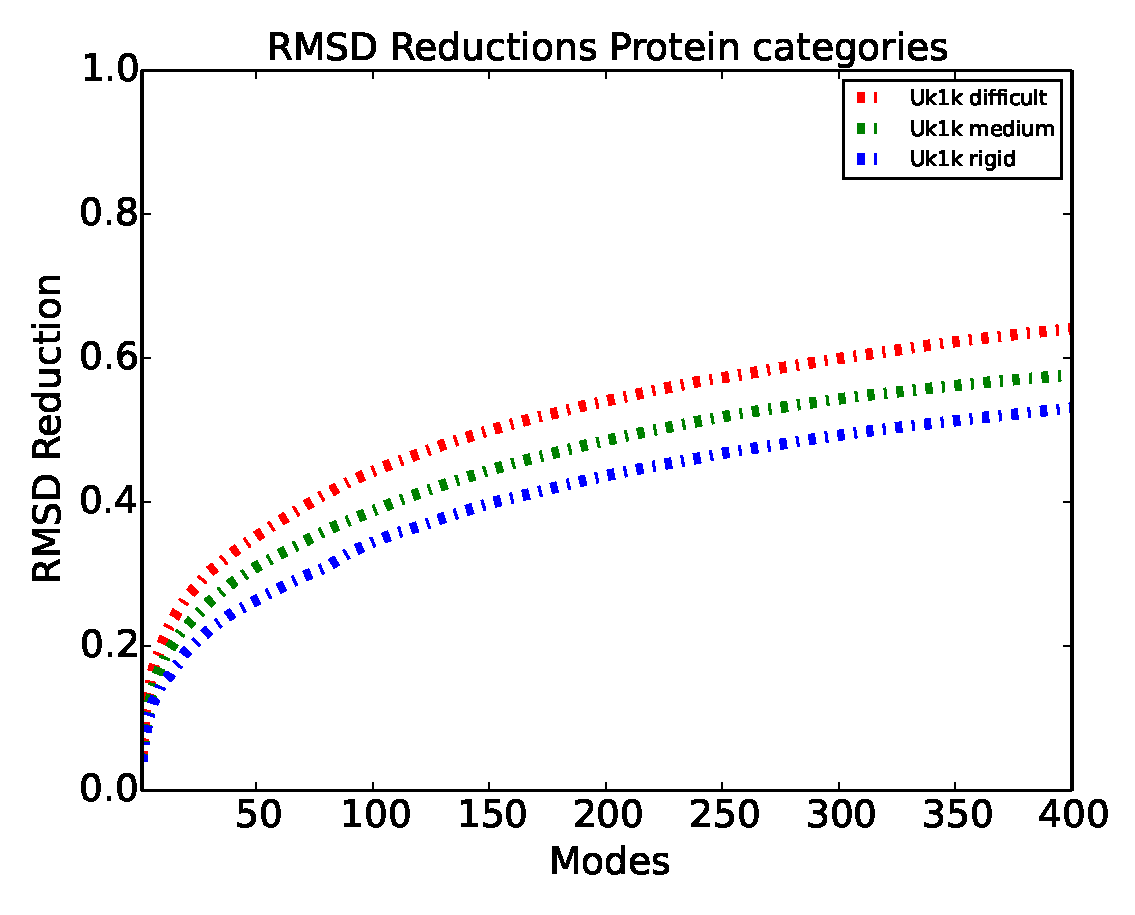
\includegraphics[width=\textwidth]{postanalysis/pics/2b_individual_canonical_whole_bb_align2bindividual_results/plots/RMSDReductionAssessmentWholeProtein.eps}
%     \caption{RMSD overall reduction}
%     \label{fig:results2plot_examplefigures2}
%     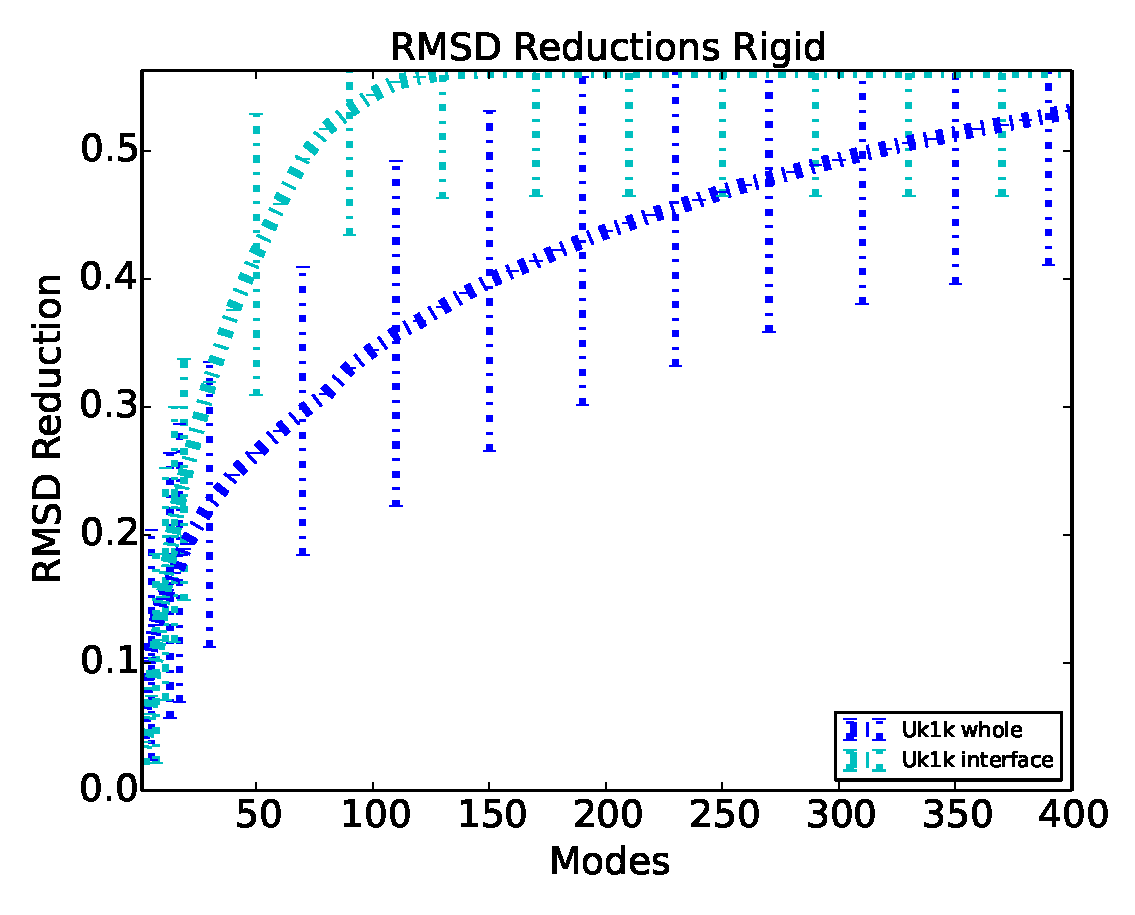
\includegraphics[width=\textwidth]{postanalysis/pics/2b_individual_canonical_whole_bb_align2bindividual_results/plots/RMSDReductionAssessmentWholeRigid.eps}
%     \caption{RMSD Reduction on the rigid cases, whole protein and interface}
%     \label{fig:results2plot_examplefigures1}
% \end{figure}

% \subsection{VarargsPlotter}
% The program ``VarargsPlotter.py'' can be used to directly plot a variable number of curves. 

% \subsection{AnalysisPlotter}
% ``AnalysisPlotter.py'' plots the experimental results specified in the input plotFile. Running it without arguments prints a help text with usage and argument descriptors

% \subsection{PostAnalysis}
% ``PostAnalysis.py'' performs the post analyis on NMA results to obtain mean and standard deviation values.

% \subsection{PostPlot}
% ``PostPlot.py'' plots the assessment output of a post analysis.

% \subsection{SuccessFailureAnalyzer \& SuccessFailurePlotter}
% ``SuccessFailureAnalyzer.py'' \& ``SuccessFailurePlotter.py'' perform the separate tasks for analyzing and plotting success-failure rates.

% \subsection{projectPDB \& projectNMD}
% ``projectPDB.py'' \& ``projectNMD.py'' can apply a transformation or projection matrix (with colums separated by a space) to a PDB/NMD file and output the resulting file.

\end{document}          
